\begin{appendices}

\setcounter{section}{0}
\renewcommand{\thesection}{SI}
%\renewcommand{\thesubsection}{SI.\arabic{subsection}}
\renewcommand{\thesubsection}{\Alph{subsection}}

\renewcommand{\thetable}{S\arabic{table}}
\setcounter{table}{0}  % Reset table counter to start from 1
\renewcommand{\thefigure}{S\arabic{figure}}
\setcounter{figure}{0}



\section{Supplemental Material}

\subsection{Data Collection}

\subsubsection{Obtaining Observational Studies}

This study adopts the definition of {\em an observational study} provided by
the NIH National Library of Medicine\footnote{https://www.ncbi.nlm.nih.gov/mesh/68064888},
which states:
``[...] a work that reports on the results of a clinical study
in which participants may receive diagnostic, therapeutic, or other types of interventions,
but the investigator does not assign participants to specific interventions (as in an interventional study).''

We initially retrieved 160,256 papers from the PubMed database using the query
{\em Observational Study[Publication Type]} via the Entrez system. The majority
of these papers were published in 2014 or later, following the
introduction of the MeSH term {\em Observational Study}. We then excluded
publications that were also labeled as {\em Randomized Controlled Trial} or {\em
Clinical Trial}, leaving us with 155,933 exclusive observational studies. Next,
we removed papers that lacked either a structured abstract with a conclusion
subsection or an English full text, resulting in 104,508 observational studies
with a {\em Conclusion(s)} subsection and English full text. Finally, we
excluded articles whose conclusions did not contain any causal or correlational
claims—typically those focused solely on descriptive findings, recommendations,
study implications, or future work. This filtering process resulted in a final
dataset of 81,132 observational studies for analysis (see
Fig.~\ref{fig__flowchart_data_collection}).


\begin{figure}[!ht]
\centering
	
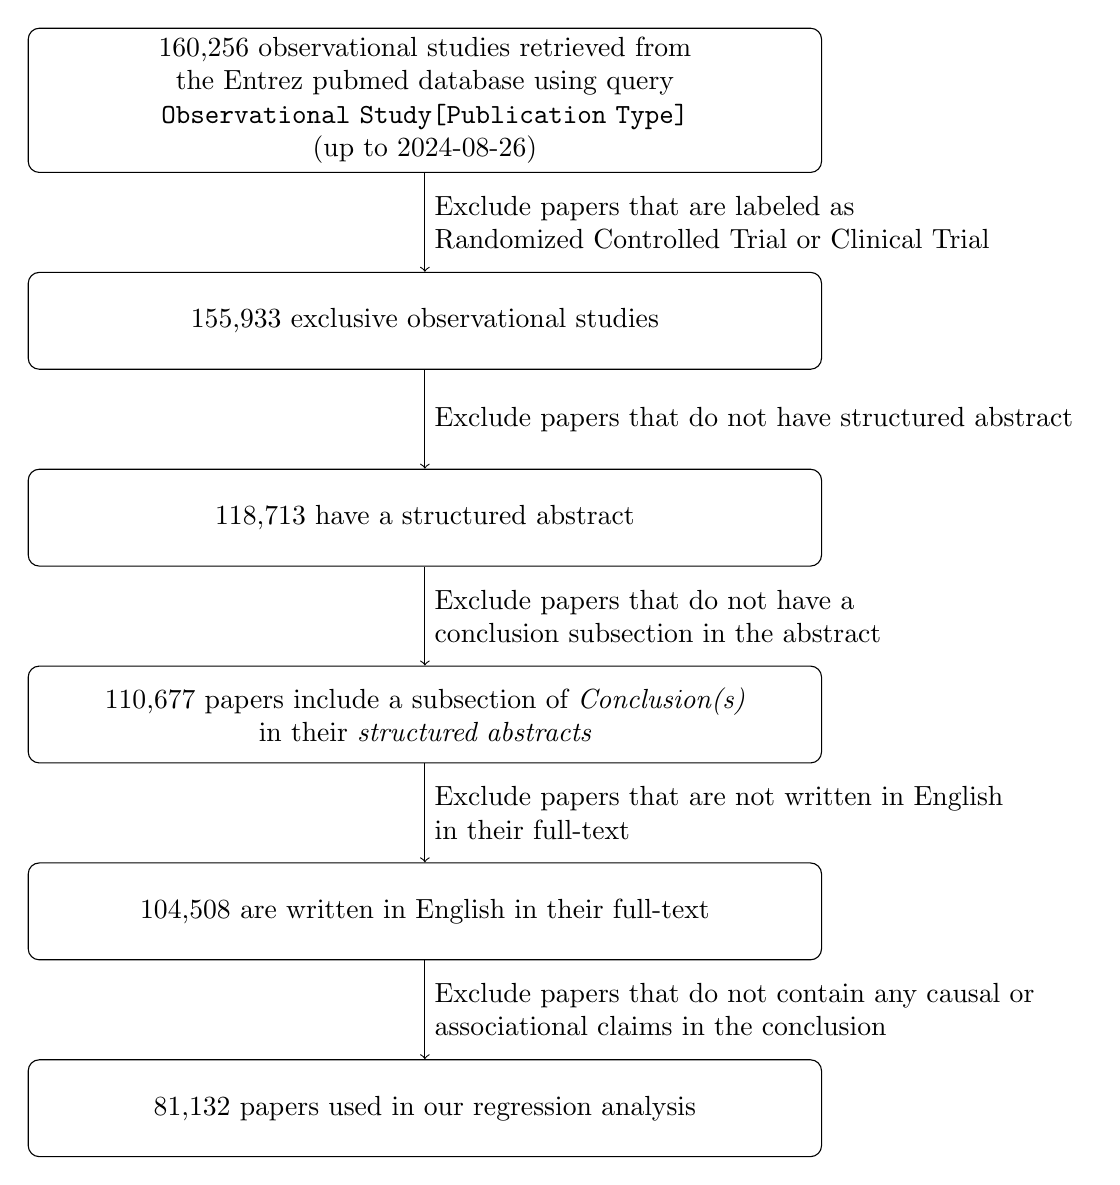
\begin{tikzpicture}
    \tikzstyle{block} = [rectangle, rounded corners, draw, text width=28em, text centered, minimum height=3.5em]

    % Place nodes
    \node [block] (block1) {160,256 observational studies retrieved from the Entrez pubmed database
    using query {\tt Observational Study[Publication Type]} \\
    (up to 2024-08-26)};
    
    \node [block, below of=block1, yshift=-1.8cm] (block2) {
        155,933 exclusive observational studies
    };
    
    \node [block, below of=block2, yshift=-1.5cm] (block2_3) {
        118,713 have a structured abstract \\ 
    };
    \node [block, below of=block2_3, yshift=-1.5cm] (block3) {
        110,677 papers include a subsection of {\em Conclusion(s)} \\ in their {\em structured abstracts}
    };
    \node [block, below of=block3, yshift=-1.5cm] (block4) {
        104,508 are written in English in their full-text
    };
    \node [block, below of=block4, yshift=-1.5cm] (block5) {
        81,132 papers used in our regression analysis
    };

    \draw[->] (block1) -- (block2) node[anchor=west, midway, align=left] {
        Exclude papers that are labeled as \\ Randomized Controlled Trial or Clinical Trial
    };
    
    \draw[->] (block2) -- (block2_3) node[anchor=west, midway, align=left] {
        Exclude papers that do not have structured abstract 
    };

    \draw[->] (block2_3) -- (block3) node[anchor=west, midway, align=left] {
        Exclude papers that do not have a \\ conclusion subsection in the abstract
    };

    \draw[->] (block3) -- (block4) node[anchor=west, midway, align=left] {
        Exclude papers that are not written in English \\ in their full-text
    };

    \draw[->] (block4) -- (block5) node[anchor=west, midway, align=left] {
        Exclude papers that do not contain any causal or \\
        associational claims in the conclusion 
    };

\end{tikzpicture}

	\caption{The process of collecting the observational studies for our analysis.}
	\label{fig__flowchart_data_collection}
\end{figure}


\subsubsection{Journal Rank}

We downloaded publicly accessible SciMago Journal Rank (SJR) data for 2023 and
prior years\footnote{https://www.scimagojr.com/journalrank.php}. For journals in
our dataset that could not be matched to the 2023 data via their ISSN, we
attempted to retrieve their information from previous years. If a journal
remained unmatched (which occurred for only 0.35\% of the papers), we assigned
it an SJR score of 0.47, corresponding to the bottom quartile in our list of
2,629 journals, based on the assumption that journals not listed in the SJR
database are likely to have a low rank.

\subsubsection{Author Writing Experience and Name Disambiguation}

An author’s writing experience is measured by the number of observational
studies they are associated with in our dataset.
To disambiguate author names, we used the
Semantic Scholar API\footnote{https://api.semanticscholar.org/} to obtain a
unique ID for each author per article. Author IDs were successfully retrieved
for 99.8\% of the authors; for the remainder, a unique random ID was generated
and assigned.



%%%%%%%%%%%%%%%%%%%%%%%
% 222
\subsection{Data Preprocessing}

\subsubsection{Causal and Correlational Claim Identification} \label{si_causal_or_correlational}

Building on our previous work  \citep{yu2019EMNLPCausalLanguage} 
and the taxonomy introduced in \citep{sumner2014association,li2017nlp}, we
curated a corpus of 3,061 sentences exemplifying causal language. Using this
dataset, we developed a BioBERT-based
model\footnote{https://github.com/junwang4/causal-language-use-in-science} to
classify a sentence in the conclusion subsection of an abstract into four levels
of claim strength: Causal, Conditional Causal, Correlational, or None. 
A “causal” claim uses terms indicating direct causation (e.g., {\em increase,
make, lead to, effective in, contribute to}) or uses the modal verb {\em can}
followed by a causal verb. A “conditional” claim uses qualifiers (e.g., {\em
may, might, appear to, probably}) to tone down the level of certainty, whereas a
“correlational” claim employs language suggesting an association (e.g., {\em
associated with, predictor, linked with}).

For this study, we merged the “conditional causal” and “correlational”
categories into a single “correlational” category, based on previous research
indicating that general readers often have difficulty distinguishing between these
two \citep{adams2017readers, bratton2020causal}. With this modification, we
fine-tuned the BioBERT-based model using the same training corpus and evaluation
procedure described in \citep{yu2019EMNLPCausalLanguage}, achieving a macro-F1
score of 0.89. Moreover, two empirical comparisons with the ChatGPT family of
models demonstrated that our specifically trained model still have advantages over ChatGPT for
this task \citep{kim2023can, chen2024evaluating}.

In our analysis, if a structured abstract’s conclusion subsection contains two
or more sentences (which occurs in 70.2\% of our dataset) and at least one
sentence is classified as causal, the entire conclusion is considered to include
a causal claim. Based on this criterion, 31.0\% of the 81,132 conclusions
contain a causal claim.

%---------------------
% 22b
\subsubsection{Country Label} \label{si_country}

Author affiliations in the PubMed metadata provide a basis for inferring country
information. However, this can be challenging when the country is not explicitly
mentioned (e.g., “Beth Israel Deaconess Medical Center”). To address this, we
developed an algorithm to infer the country associated with an author’s
affiliation, trained on a dataset of 2.7 million organizations with known
country information from the ORCID
database\footnote{https://support.orcid.org/hc/en-us/articles/360006897394-How-do-I-get-the-public-data-file}.

We evaluated the algorithm using 1,000 randomly sampled affiliations from the
PubMed metadata. These affiliations fell into two categories: (1) those with
insufficient information to infer the country (e.g., “Division of Infectious
Diseases”) and (2) those with sufficient information. For the few cases (7
affiliations) in Category 1, the algorithm output low confidence (less than
0.8), whereas for Category 2, all inferences were accurate. For additional
details, please visit our GitHub
page\footnote{https://github.com/junwang4/affiliation-to-country-inference}.

For each paper, if all author affiliations are classified under the same country
and the average confidence score exceeds 0.8, the paper is labeled with that
country; otherwise, it is labeled as “others.”
Fig.~\ref{fig__country_distribution} shows the distribution of countries that
have published at least 300 observational studies.

\begin{figure}[!ht]
    \includegraphics[width=.9\textwidth]{./figure/country_distri_R.pdf}
        \caption{
        Number of observational studies by authors from 27 exclusive countries that
        have published at least 300 papers in our dataset, along with the “others” category.
        The “others” category includes 23,153 observational studies: 
        15,906 from multiple countries,
         4,931 from various other countries 
         (each with fewer than 300 studies published),
          1,539 lacking affiliation data,
           and 777 with low-confidence inference (i.e., confidence less than 0.8).
        }
        \label{fig__country_distribution}
    \end{figure}


%---------------------
% 22c
\subsubsection{Gender Label} \label{si_gender}

Gender is inferred from an author's forename. Using a dataset of 6 million
(forename, gender) pairs from WikiData, we developed a Gradient Boosting-based
algorithm that leverages the last eight letters of forenames as features to
predict the likelihood that a name is male or female.

Our algorithm\footnote{https://github.com/junwang4/name-to-gender-inference}
performs comparably to the best of the five name-to-gender inference tools when
evaluated on a benchmark dataset of 5,779 manually labeled names
\citep{Santamara2018ComparisonAB}. In our implementation, a name is labeled as
male if its male confidence exceeds 0.83 and as female if its female confidence
exceeds 0.71; otherwise, it is classified as gender-unknown. These thresholds
achieve balanced recall (0.86 for both male and female) and high precision (0.98
for male and 0.97 for female). Note that the lower threshold for females
reflects the fact that 75\% of the training data comprises male names.

Fig.~\ref{fig__gender_distribution} illustrates the gender distribution among
first and last authors. The pattern, where men outnumber women in both
roles, aligns with prior reports of gender imbalances in biomedical research
publications \citep{ioannidis2023gender}, 
with a more noticeable difference observed among last authors (about 2.5 men per woman).


\begin{figure}[!ht]
    \centering
    \begin{subfigure}{\textwidth}
        \centering
        \includegraphics[width=0.45\textwidth]{./figure/gender_distribution.pdf}
    \caption{Gender distribution by author position. F: female; M: male; I:
    initials only; L: low-confidence inference. For first authors, 37.4\% of
    non-initial forenames are identified as female and 52.3\% as male; for last
    authors, 25.1\% are female and 65.6\% are male. Cases with initials only or
    low-confidence inferences are combined as gender-unknown, comprising 16.9\%
    of first authors and 16.2\% of last authors.}
        \label{fig__gender_distribution_1}
    \end{subfigure}
    \hfill
    \begin{subfigure}{\textwidth}
        \centering
        \includegraphics[width=\textwidth]{./figure/country_gender_firstlast_distri_R.pdf}  % Replace with your image path
	\caption{
      Gender distribution by country (after combining genders of first and last
      authors). F: female; M: male; I: initials only; L: low-confidence
      inference. For mainland China (CN), South Korea (KR), and Taiwan (TW),
      approximately half of the names are difficult to infer from the forename
      alone.
      }
        \label{fig__gender_distribution_2}
    \end{subfigure}

    \caption{Gender distribution}
    \label{fig__gender_distribution}
\end{figure}


\newpage

%%%%%%%%%%%%%%%%%%%%%%%
% 333
\subsection{Logistic Linear Mixed-Effects Regression Analysis}

%\newcommand{\ttt}{\texttt\footnotesize}

\begin{table}[ht]
    \centering
%\Large
    \begin{tabular}{@{}ll@{ }ll@{}}
        %\multicolumn{4}{l}{\large Does\_The\_Observational\_Study\_Use\_Causal\_Claim\_In\_Its\_Abstract\_Conclusion$\sim$} \\ [.1in]
        %\multicolumn{4}{l}{\large Has\_causal\_claim\_in\_abstract\_conclusion $\sim$} \\ [.2in]
        \multicolumn{4}{l}{\large Has\_causal\_language\_use\_in\_the\_conclusion\_of\_a\_structured\_abstract $\sim$} \\ [.2in]

       % &&  $\sum_i StudyCharacteristics_i$ &  {\ttt// $i\in$\{Observational, Comparative, Multicenter, Systematic Review, Validation, Evaluation, Case Reports\}} \\

%& &   $\sum_i StudyDesign_i$ & {\ttt // $i\in$\{Retrospective, Prospective, Case-Control, Cross-Sectional, Cohort, Follow-Up, Longitudinal\}}\\

        & \multicolumn{3}{l}{\ttt \large // VARIABLES OF INTEREST} \\ [.1in]
        &  & Num\_coauthors &   {\ttt // log-scaled}  \\
        & + & Num\_obs\_studies\_by\_{\bf first}\_author &  {\ttt// log-scaled} \\
        & + & Num\_obs\_studies\_by\_{\bf last}\_author &  {\ttt// log-scaled} \\
        & + & Gender\_of\_{\bf first}\_author & {\ttt // categorical: F, M, Unknown} \\
        & + & Gender\_of\_{\bf last}\_author & {\ttt // categorical: F, M, Unknown} \\
        & + & Country\_of\_authors & {\ttt// categorical: 27 exclusive countries and others}\\ [.2in]

    & \multicolumn{3}{l}{\ttt \large // CONTROL VARIABLES} \\ [.1in]
        & + & Journal\_rank &   {\ttt// log-scaled: Scimago journal rank}  \\
        & + & Num\_obs\_studies\_in\_the\_journal &   {\ttt// log-scaled}  \\
        & +& $\sum_{i=1}^{N} \textrm{MeSH\_term}_i$  & {\ttt // binary: N$=$771 MeSH terms, each with at least 150 papers} \\[.2in]

    & \multicolumn{3}{l}{\ttt \large // RANDOM EFFECT VARIABLES} \\ [.1in]
& + & (1 $|$ Year) & {\ttt // categorical: the majority are from 2013 to 2024} \\
& + & (1 $|$ Journal) & {\ttt// categorical: 2629 journals} \\  
& + & (1 $|$ Num\_sentences\_in\_the\_conclusion) &  {\ttt// categorical: the majority are 1, 2, or 3 sentences}
\\ [.2in]
\end{tabular}
\caption{
The formula for the logistic linear mixed-effects regression model.
}
\label{tab_modelformula}
\end{table}



The results presented in Table~\ref{table__overall_effects} are based on a
logistic linear mixed-effects regression model (formula provided in
Table~\ref{tab_modelformula}). Specifically, we used the $glmer()$ function from
the R package $lme4$ \citep{Bates2014FittingLM} on 81,132 observations. In our
model, the dependent variable indicates whether the conclusion subsection of an
article's structured abstract contains at least one sentence with a causal
claim. The primary explanatory variables include: (1) Author writing experience
(measured as the number of observational studies published by the first/last
authors, log-transformed to address skewness); (2) Author gender (for first and
last authors); (3) Author country; and (4) Team size (the number of authors,
also log-transformed).



\subsection{Effects of Various Research Topics, Methods, and Concepts} \label{meshtermeffect}

Our dataset contains over 771 Medical Subject Headings (MeSH) terms, each
treated as a control variable, with its absence serving as the reference
category. A MeSH term is included if it is assigned to at least 150 articles in
the dataset and is not a country name (since author country is analyzed
separately). Table~\ref{meshtermeffect} reports the effects of these MeSH terms,
ordered by effect size.

Refer to the following GitHub repository for a detailed report on the effects of
these MeSH terms.

\noindent\href{https://github.com/junwang4/causal-language-use-80k-observational-studies/blob/main/pdf/meshterm_effects.pdf}{https://github.com/junwang4/causal-language-use-80k-observational-studies}

\end{appendices}